%%%% ijcai18.tex

\typeout{IJCAI-18 Instructions for Authors}

% These are the instructions for authors for IJCAI-18.

\documentclass{article}
\pdfpagewidth=8.5in
\pdfpageheight=11in
% The file ijcai18.sty is the style file for IJCAI-18 (same as ijcai08.sty).
\usepackage{ijcai18}

% Use the postscript times font!
\usepackage{times}
\usepackage{soul}
\usepackage{url}
\usepackage[hidelinks]{hyperref}
\usepackage[utf8]{inputenc}
\usepackage[small]{caption}
\usepackage{float}
\usepackage{multirow}
\usepackage{amsmath,amsthm,amsfonts}
\usepackage{array}
\usepackage{algorithm}
\usepackage[noend]{algpseudocode}
\usepackage{graphicx}
\usepackage{tikz}
\usepackage{pgfplots}
\usepackage{textcomp}
\usepackage{tikz}
\usetikzlibrary{shapes,backgrounds}
\renewcommand{\arraystretch}{1.4}
\graphicspath{ {images/} }
\usepackage{tikz-qtree,tikz-qtree-compat}
% the following package is optional:
%\usepackage{latexsym} 

% Following comment is from ijcai97-submit.tex:
% The preparation of these files was supported by Schlumberger Palo Alto
% Research, AT\&T Bell Laboratories, and Morgan Kaufmann Publishers.
% Shirley Jowell, of Morgan Kaufmann Publishers, and Peter F.
% Patel-Schneider, of AT\&T Bell Laboratories collaborated on their
% preparation.

% These instructions can be modified and used in other conferences as long
% as credit to the authors and supporting agencies is retained, this notice
% is not changed, and further modification or reuse is not restricted.
% Neither Shirley Jowell nor Peter F. Patel-Schneider can be listed as
% contacts for providing assistance without their prior permission.

% To use for other conferences, change references to files and the
% conference appropriate and use other authors, contacts, publishers, and
% organizations.
% Also change the deadline and address for returning papers and the length and
% page charge instructions.
% Put where the files are available in the appropriate places.

\usepackage{xcolor,colortbl}
\newcommand{\mohit}[1]{{\bf \textcolor{blue}{{Mohit: #1}}}}
\newcommand{\luc}[1]{{\bf \textcolor{red}{{Luc: #1}}}}
\newcommand{\stefano}[1]{{\bf \textcolor{violet}{{Stefano: #1}}}}

\usepackage{xspace}
\newcommand{\learner}{\textsc{NL-CountOR}}
\newcommand{\TX}{\textbf{X}\xspace}
\newcommand{\TY}{\textbf{Y}\xspace}
\newcommand{\TZ}{\textbf{Z}\xspace}
\newcommand{\TP}{\textbf{P}\xspace}
\newcommand{\TM}{\textbf{M}\xspace}
\newcommand{\TN}{\textbf{N}\xspace}
\newcommand{\TE}{\textbf{E}\xspace}
\newcommand{\TF}{\textbf{F}\xspace}
%\newcommand{\TH}{\textbf{H}}
\newcommand{\Nonzero}[2]{\text{Nonzero}\!\left(#1,#2\right)}
\newcommand{\Sum}[2]{\text{Sum}\!\left(#1,#2\right)}
\newcommand{\MaxConsOne}[2]{\text{MaxConsOne}\!\left(#1,#2\right)}
\newcommand{\MinConsOne}[2]{\text{MinConsOne}\!\left(#1,#2\right)}
\newcommand{\MaxConsZero}[2]{\text{MaxConsZero}\!\left(#1,#2\right)}
\newcommand{\MinConsZero}[2]{\text{MinConsZero}\!\left(#1,#2\right)}
\newcommand{\Count}[3]{\text{Count}\!\left(#1,#2,#3\right)}

\newcommand{\Nurses}{\texttt{Nurses}}
\newcommand{\Shifts}{\texttt{Shifts}}
\newcommand{\Days}{\texttt{Days}}
\newcommand{\Nurse}{\texttt{Nurse}}
\newcommand{\Shift}{\texttt{Shift}}
\newcommand{\Day}{\texttt{Day}}

%\usepackage{etoolbox}
%\let\bbordermatrix\bordermatrix
%\patchcmd{\bbordermatrix}{8.75}{4.75}{}{}
%\patchcmd{\bbordermatrix}{\left(}{\left[}{}{}
%\patchcmd{\bbordermatrix}{\right)}{\right]}{}{}

\newcommand{\mc}[2]{\multicolumn{#1}{c}{#2}}
\definecolor{Colored}{rgb}{0.85,0.85,0}
\newcolumntype{a}{>{\columncolor{Colored}}c}


\title{Learning Non-Linear Constraints using Tensors}
\author{
Mohit Kumar$^1$,
Stefano Teso$^1$,
Luc De Raedt$^1$
\\ 
$^1$ KU Leuven\\
%
\texttt{\{mohit.kumar,stefano.teso,luc.deraedt\}@cs.kuleuven.be}
}
% If your authors do not fit in the default space, you can increase it 
% by uncommenting the following (adjust the "2.5in" size to make it fit
% properly)
% \setlength\titlebox{2.5in}


\begin{document}

\maketitle

\begin{abstract}
Many problems in operations research require that constraints be specified in the model. Determining the right constraints is a hard and laborsome task.
We propose an approach to automate this process using artificial intelligence and machine learning principles. So far there has been only little work on learning constraints within the operations research community.
We focus on personnel rostering and scheduling problems in which there are often past schedules available and show that it is possible to automatically learn  constraints from such examples. 
To realize this, we adapted some techniques from the constraint programming community and  we have extended them in order to  cope with multidimensional examples. 
The method uses a tensor representation of the example, which helps in capturing the dimensionality as well as the structure of the example, and applies tensor operations to find the constraints that are satisfied by the example. 
To evaluate the proposed algorithm, we used constraints from the Nurse Rostering Competition and generated solutions that satisfy these constraints; these  solutions were then used as examples to learn constraints. Experiments demonstrate that the proposed algorithm is capable of producing human readable constraints that capture the underlying characteristics of the examples. 
\end{abstract}


\section{Introduction}
\label{sec:intro}

%\begin{itemize}
%\item Do not 
%\end{itemize}

%
%
%%\begin{columns}
%%\begin{column}{width=0.1\textwidth}
%%X = 
%%\end{column}
%%\begin{column}{0.5\textwidth}
%\begin{table}[t]
%\begin{small}
%    \begin{center} 
%        \begin{tabular}{c|c|c|c|c|c|c|c|c|c|}
%            \cline{2-10}
%            \multicolumn{1}{l|}{}                  & \multicolumn{3}{c|}{$\text{Day}_1$} & \multicolumn{3}{c|}{$\text{Day}_2$} & \multicolumn{3}{c|}{$\text{Day}_3$} \\
%            \cline{2-10}
%            \multicolumn{1}{l|}{}                  & $\text{S}_1$     & $\text{S}_2$     & $\text{S}_3$     & $\text{S}_1$     & $\text{S}_2$     & $\text{S}_3$     & $\text{S}_1$     & $\text{S}_2$     & $\text{S}_3$ \\
%            \hline
%            \multicolumn{1}{|c|}{$\text{Nurse}_1$} &  1      &  0      &  0      & 0      & 1      & 0      & 0      & 1      & 0 \\
%            \hline
%            \multicolumn{1}{|c|}{$\text{Nurse}_2$} & 0      & 1      & 0      & 1      & 0      & 0      & 0      & 0      & 1 \\
%            \hline
%            \multicolumn{1}{|c|}{$\text{Nurse}_3$} & 0      & 0      & 1      & 0      & 0      & 0      & 1      & 0      & 0 \\
%            \hline
%            \multicolumn{1}{|c|}{$\text{Nurse}_4$} & 0      & 0      & 1      & 0      & 0      & 1      & 1      & 0      & 0 \\
%            \hline
%        \end{tabular}
%    \end{center}
%%    \caption{\label{tab:dataformat} Example nurse schedule with three dimensions: four nurses, three days, and three shifts per day.}
%\end{small}
%\end{table}
%%\end{column}
%%\end{columns}


% \stefano{@Mohit: please go through the paper and remove all references to ``data''.  We work with examples, solutions, candidate constraints, constraints, and models.  ``Data'' is confusing.}

Constraints are pervasive in practical scheduling and rostering problems. For example, hospitals usually generate a weekly schedule for their nurses based on constraints like the maximum number of working days for a nurse. As the number of nurses and the complexity of the constraints increases, however, generating the schedule manually becomes impossible.  Organizations may hire domain experts to manually model the constraints, but this is expensive and time consuming. A tempting alternative is to employ constraint learning~\cite{de2018learning} to automatically induce the constraints from examples of past schedules.

Unfortunately, existing constraint learners are not tailored for this setting.  Classical approaches like Conacq~\cite{Bessiere} and Inductive Logic Programming tools~\cite{MUGGLETON1994629} focus on logical variables only,  while scheduling constraints often include numerical terms.  Very few approaches can handle this case.  TaCLe~\cite{kolb2017learning} focuses on 2-D tabular data (Excel spreadsheets), while schedules are inherently multi-dimensional. To see what we mean, consider the nurse schedule shown in Table~\ref{tab:dataformat}.  For each combination of nurse, day and shift the value of 1 represents that the nurse worked in that particular shift of that day, while a 0 means the nurse didn't work.  It is easy to see that nurses, days, and shifts are independent of each and behave like different dimensions.  ModelSeeker~\cite{beldiceanu2012model} is the only method that can handle such multi-dimensional structures, but it is restricted to global constraints only.

%Learning constraints like ``the minimum/maximum number of people working each day'' is not trivial.  Doing so requires to check, for each nurse and day whether they worked in any of the 3 shifts, and represent it by 1 or 0, which is like taking a vector of size 3 (corresponding to the 3 shifts) and reducing it to a scalar value of 1 or 0\stefano{@Mohit: $\gets$ very unclear}. Existing constraint learners are not equipped for dealing with this.

To address this issue, we propose COnstraint UsiNg TensORs (\learner{}), a novel constraint learning approach that leverages tensors for capturing the inherent structure and dimensionality of the schedules.  In order to learn the constraints, \learner{} extracts and enumerates all (meaningful) slices of the input schedule(s), aggregates them through tensor operations, and then computes bounds for the aggregates to generate candidate numerical constraints.  Some simple filtering strategies are applied to prune irrelevant and trivially satisfied candidates.  When increasing the number of dimensions in the example, the rank of the tensor representing the example will increase accordingly but the proposed method \learner{} remains unchanged, so \learner{} can easily scale to large and complex schedules. The number of candidate sub-tensors however increases exponentially with the number of dimensions of $\TX$.

We make the following key contributions:
%
(\textbf{1}) A tensor representation of schedules and constraints appropriate for real-world personnel rostering problems.
%
(\textbf{2}) A novel constraint learning algorithm, \learner{}, which uses tensor extraction and aggregation operations to learn the constraints hidden in the input schedules.
%and also filter out the constraints which doesn't make much sense.
%
(\textbf{3}) An empirical evaluation on real-world nurse rostering problems.
%
%(\textbf{4}) An extension of \learner{} to the case where additional background knowledge (e.g. nurse skill levels) are available.

The paper is structured as follows. We present the method in Section~\ref{sec:method}, followed by evaluation on example instances  in Section~\ref{sec:experiments}. We conclude with some final remarks in Section~\ref{sec:conclusion}.


% \section{Method}
% \label{sec:method}

% We looked into most of the benchmark scheduling problems prevailing in the operations research community, some examples are Nurse Rostering, Course Timetabling, Home Care Scheduling and Project Scheduling. Most of the constraints observed in these problems are non-linear in nature but share some kind of structure, so we did some deep dive and came up with a mathematical structure to represent most of these constraints. 

% Let's see this running example before we define this structure. Consider a Nurse rostering model with the following variables.
% %
% \begin{align*}
%   \TX_{n,s,d} = & \begin{cases}
%     1, & \text{if nurse $n$ is allocated shift $s$ on day $d$}\\
%     0, & \text{otherwise}.
%   \end{cases}\\
%   \textbf{H}_{n} = & \begin{cases}
%     1, & \text{if nurse $n$ is high skilled}.\\
%     0, & \text{otherwise}.
%   \end{cases}\\
%   \textbf{M}_{n} = & \begin{cases}
%     1, & \text{if nurse $n$ is medium skilled}.\\
%     0, & \text{otherwise}.
%   \end{cases}\\
%   \textbf{L}_{n} = & \begin{cases}
%     1, & \text{if nurse $n$ is low skilled}.\\
%     0, & \text{otherwise}.
%   \end{cases}\\
%   \textbf{R}_{s,d} =
%     & \; \text{Minimum number of high or medium skilled}\\ 
%     & \; \text{nurses required in shift $s$ on day $d$}
% \end{align*}
% %
% Considering these variables, a constraint like "the minimum number of high or medium skilled nurses working in a shift" can be represented as:
% \begin{equation}
% \label{eq:const}
% \sum_{n} \TX_{n,s,d} \times \textbf{H}_{n} + \sum_{n} \TX_{n,s,d} \times \textbf{M}_{n} \geq \textbf{R}_{s,d} \quad \forall s,d
% \end{equation}
% %
% A generic version of the constraint above is represented below (Eq~\ref{eq:struct}).
% Let $\mathbb{X}$ represents the set of all tensors 
% %\stefano{@Mohit: maybe it's best to differentiate between tensors, written \TX, and sets of tensors, say, $\mathbb{X}$?} 
% $\TP(\mathbb{X})$ represents the power set of $\mathbb{X}$ and $\TE,\TF \subseteq \TP(\mathbb{X})$.
% %Let $j$ represents the index set for $\TE$ and $i$ represents the index set for elements in \TE.
% %$J \subseteq \{1,2,...,|P|\}$.
% \begin{multline}
% \label{eq:struct}
% 	\displaystyle\sum\limits_{\textbf{e} \in \TE}(\sum_{S_e}\prod_{\TY \in \textbf{e}} \TY_{M_{e,y}}) 
% 	-\sum\limits_{\textbf{e'} \in \TE'}(\sum_{S_{e'}}\prod_{\TY \in \textbf{e'}} \TY_{M_{e',y}}) \le \TZ_{M}\\
% 	\forall \bigcup_{l \in E \cup E'}(\bigcup_{\TY \in \textbf{l}} M_{l,y} / S_l) \bigcup M
% \end{multline}
% Each constraint in Eq~\ref{eq:struct} can be uniquely identified by the following variables:
% \begin{itemize}
% \item $E, E', Z$
% \item $M_{l,y} \quad \forall l \in E \bigcup F \quad and\quad  y \in l$
% \item $S_{l} \quad \forall l \in E \bigcup F$
% \item $M$
% \end{itemize}
% In other words, by enumerating through the various possible values of these variables, we can enumerate through all the possible constraints. For example, choosing the following assignments will give us the constraint represented by Eq~\ref{eq:const}
% \begin{align*}
% &E=\emptyset\\
% &F=\{(X,H),(X,M)\}\\
% &Z=R\\
% &M_{(X,H),X}=M_{(X,M),X}=\{n,s,d\}\\
% &M_{(X,H),H}=M_{(X,M),M}=\{n\}\\
% &S_{(X,H)}=S_{(X,M)}=\{n\}\\
% &M=\{s,d\}
% \end{align*}
% Enumerating through all the possible combinations is not a feasible solution as the number of combinations for this structure is huge and enumerating through all the possibilities will not scale for the real world problems. In this paper we define a two step solution to tackle this problem:


\section{Method}
\label{sec:method}

Most of the constraints in the prevalant benchmark scheduling problems are non-linear in nature and share an inherent structure. In this paper, we first define a mathematical structure to represent these constraints and then define an algorithm to learn these structures efficiently. Thus automating the rigourous task of desiging and coding constraints to reach the solution.
%We looked into most of the benchmark scheduling problems prevailing in the operations research community, some examples are Nurse Rostering, Course Timetabling, Home Care Scheduling and Project Scheduling. Most of the constraints observed in these problems are non-linear in nature but share some kind of structure, so we did some deep dive and came up with a mathematical structure to represent most of these constraints. 

We introduce a running example before delving into more details. Consider a Nurse rostering model with the following variables.
%
\begin{align*}
  \TX_{n,s,d} = & \begin{cases}
    1, & \text{if nurse $n$ is allocated shift $s$ on day $d$}\\
    0, & \text{otherwise}.
  \end{cases}\\
  \textbf{H}_{n} = & \begin{cases}
    1, & \text{if nurse $n$ is high skilled}.\\
    0, & \text{otherwise}.
  \end{cases}\\
  \textbf{M}_{n} = & \begin{cases}
    1, & \text{if nurse $n$ is medium skilled}.\\
    0, & \text{otherwise}.
  \end{cases}\\
  \textbf{L}_{n} = & \begin{cases}
    1, & \text{if nurse $n$ is low skilled}.\\
    0, & \text{otherwise}.
  \end{cases}\\
  \textbf{R}_{s,d} =
    & \; \text{Maximum number of high or medium skilled}\\ 
    & \; \text{nurses required in shift $s$ on day $d$}
\end{align*}
%
Considering these variables, a constraint like "the maximum number of high or medium skilled nurses working in a shift" can be represented as:
\begin{equation}
\label{eq:const}
\sum_{n} \TX_{n,s,d} \times \textbf{H}_{n} + \sum_{n} \TX_{n,s,d} \times \textbf{M}_{n} \le \textbf{R}_{s,d} \quad \forall s,d
\end{equation}
Each term in the left hand side of Eq~\ref{eq:const} can be represented by:
\begin{equation}
\label{eq:struct}
	\bigotimes_{\textbf{S}}(\overline{\TX}, \overline{\TM}) = \sum_{\textbf{S}}\prod_{\TX,\TM \in \overline{\TX} \odot \overline{\TM}}\TX_{\TM}
\end{equation}
Here, $\odot$ is an element wise concatenation, for example: {\mohit{needs fixing}}
\begin{equation*}
    \{X_1,X_2\}\odot \{M_1,M_2\}=\{(X_1, M_1), (X_2, M_2)\}
\end{equation*}
Taking $\overline{\TX}=\{\TX_{n,s,d}, \textbf{H}_{n}\}$, $\overline{\TM}=\{\{n,s,d\}, \{n\}\}$ and $\textbf{S}=\{n\}$ will give us the first term in Eq~\ref{eq:const}, i.e. 
$\bigotimes_{\textbf{S}}(\overline{\TX}, \overline{\TM})=\sum_{n} \TX_{n,s,d} \times \textbf{H}_{n}$.
\\
Let $\mathbb{X}$ represents the set of all tensors, $\TP(\mathbb{X})$ represents the power set of $\mathbb{X}$ and $\TE \subseteq \TP(\mathbb{X})$, then the following inequality captures the type of constraint we saw in Eq~\ref{eq:const}.
%Let $j$ represents the index set for $\TE$ and $i$ represents the index set for elements in \TE.
%$J \subseteq \{1,2,...,|P|\}$.
\begin{multline}
\label{eq:struct}
	\displaystyle\sum\limits_{\overline{\TX}_i \in \TE}\bigotimes_{\textbf{S}_i}(\overline{\TX}_i,\overline{\TM}_i) \le \TZ_{M}\\ \forall \bigcup_{i}(\bigcup_{\TM \in \overline{\TM}_i} \TM / \textbf{S}_i) \bigcup M 
\end{multline}
Each constraint in Eq~\ref{eq:struct} can be uniquely identified by the following parameters:
\begin{itemize}
\item $\TE, \overline{\TM}_i,\textbf{S}_i, \TZ, \TM$
\end{itemize}
For example, choosing the following assignments will give us the constraint represented by Eq~\ref{eq:const}
\begin{align*}
&E=\{(X,H),(X,M)\}\\
&Z=R\\
&\overline{M}_{(X,H)}=\overline{M}_{(X,M)}=\{(n,s,d), (n)\}\\
&S_{(X,H)}=S_{(X,M)}=\{n\}\\
&M=\{s,d\}
\end{align*}
By enumerating through the possible values of these variables, we can enumerate through all the possible constraints. However, that is not a feasible solution, as the number of combinations for this structure is huge and enumerating through all the possibilities will not scale for the real world problems. In this paper we define a two step solution to tackle this problem:

\subsection{Signatures}
Signatures are a pro active measure to refine the set of constraints to be enumerated. We define the following conditions which must be satisfied by a constraint in order for it to be a valid constraint. Let $N_y$ represents the dimension set of \TY
\begin{itemize}
            \item $M_{l,y} \subseteq N_y \quad \forall l \in E \bigcup F$
            \item $S_{l} \subseteq \bigcup_{\TY \in l} M_{l,y}$ for all $l \in E \bigcup F$
            \item $\bigcup_{\TY \in l} M_{l,y} / S_{l} = \bigcup_{\TY \in l'} M_{l,y} / S_{l'}\quad \forall l,l' \in E \bigcup F$
            \item $\bigcup_{\TY \in l} M_{l,y} / S_{l} \subseteq M$ or
            $\bigcup_{\TY \in l} M_{l,y} / S_{l} \supseteq M\quad \forall l \in E \bigcup F$
            
%            \item $M_{l,y} = N_y \quad \forall l \in E \bigcup F$
            \item $\TY \ne \TY'$ for any $\TY,\TY' \in l \quad \forall l \in E \bigcup F$
            \item $|E|+|F| \le 2$
            \item $|l| \le 2\quad \forall l \in E \bigcup F$
            % \item $a-b \le 0$
\end{itemize}
If we apply just the last two signatures to Eq~\ref{eq:struct}, the structure reduces to:
\begin{equation}
\label{eq:one}
	\displaystyle\sum_{S} \TX_{M_1} *\TY_{M_2}
	+\sum_{S'} \TX'_{M'_1} *\TY'_{M'_2} \le \TZ_{M}
\end{equation}
\begin{equation}
\label{eq:two}
	\displaystyle\sum_{S} \TX_{M_1} *\TY_{M_2}
	+\sum_{S'} \TX'_{M'_1} *\TY'_{M'_2} \geq \TZ_{M}
\end{equation}
\begin{equation}
\label{eq:three}
	\displaystyle\sum_{S} \TX_{M_1} *\TY_{M_2}
	-\sum_{S'} \TX'_{M'_1} *\TY'_{M'_2} \le \TZ_{M}
\end{equation}

\subsection{Intelligent Enumeration}
\begin{figure}[tb]
    \centering
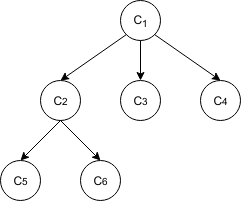
\includegraphics[width=0.3\textwidth]{images/constraintTree.png}
    \caption{\label{fig:constraintTree} Constraint Dependency Tree: The root represents the most general constraint and as we keep going down the constraints become more specific.}
\end{figure}
This subsection presents an intelligent way to enumerate through constraints based on the concept of logical entailment. We define a constraint dependency tree as shown in Fig~\ref{fig:constraintTree}. Each node in this tree represents costraint and a directed edge between two nodes represent entailment. For example, in Fig~\ref{fig:constraintTree}, $C_2$ entails $C_1$ which means whenever $C_2$ is satisfied $C_1$ will also be satisfied, which also means if $C_1$ is not satisfied then $C_2$ is not satisfied either.
There are two ways to enumerate using this tree:
 
\textbf{Top Down:} In the top down approach, we start with the most general constraint, if it's not satisfied then we don't need to check any of it's descendents. For example, in Fig~\ref{fig:constraintTree}, we start with checking the validity of $C_1$, if it is not satisfied we don't need to check any other constraints in the tree as none of them would be satisfied, and if it's not then we check each of it's children one by one and repeat the process.

\textbf{Bottom Up:} Bottom up works on the similar idea as the top down approach, here we start with the most specific constraint, in our case it would be $C_5$ or $C_6$, if it is satisfied we don't need to check any ancestors of that constraint as it will definitely be satisfied, but if it's not satisfied we check each parent one by one and repeat the process.

In this paper we are going to discuss top down approach, but we can easily transform the algorithm to consider the bottom up approach. 
\\
To build a constraint dependency tree, we define the entailment properties for the operations used while constructing a constraint using Eq~\ref{eq:struct}: Summation over terms($S_t$), summation over dimensions($S_d$), product($P$) and slicing($S$). Except slicing all three operations can be used to define entailment:
\begin{itemize}
\item $X \not\le Z \Rightarrow X + Y \not\le Z \quad \forall Y \geq 0$
\item $X_{M} \not\le Z \Rightarrow X_{M'} \not\le Z \quad \forall M': M' \supset M \, and \, X \geq 0$
\item $X \not\le Z \Rightarrow X * Y \not\le Z \quad \forall Y: Y \geq 1$
\item $X + Y \not\le Z \Rightarrow X \not\le Z \quad \forall Y \le 0$
\item $X_{M} \not\le Z \Rightarrow X_{M'} \not\le Z \quad \forall M': M' \subset M \, and \, X \le 0$
\item $X * Y \not\le Z \Rightarrow X \not\le Z \quad \forall Y: Y \le -1$
\end{itemize}


To use these properties, we have to make some assumptions. We start by using the first three property to define a simple algorithm which gives an idea of how the algorithm works. Thereafter, we keep on relaxing the assumptions we made and explain how the algorithm changes for the revised structure to use the other properties given above. The first two properties can only be used if all the entries in the tensors are non-negative, while for the third one we need the values to be greater than or equal to 1. So for now we assume the values in each tensor to be greater than or equal to 1
%So, the initial assumption is:
%\begin{itemize}
%\item Mod of the numbers in a tensor is always greater than or equal to 1
%\item Each tensor has only non-negative entry.
%\end{itemize}
% With the first assumption in place and given the structure of the constraints that we enumerate using Eq~\ref{eq:struct}, we can safely assume that all the tensors have only positive numbers. This is because even if we have any negative data tensor \textbf{T}, we can transform it to \textbf{-T} for our algorithm without loosing any information as our equation considers both \textbf{T} and \textbf{-T} when enumerating through constraints.
%Combining both the assumptions we can say that each number in each tensor must be greater than or equal to 1. 

% \begin{equation}
% t_1 \not\ge t \implies t_1 * t_2 \not\ge t \quad \forall t_2, s.t. |t_2| \le 1
% \end{equation} 

To use the bottom up approach, we first define what the most specific constraints (the root nodes) look like and then define the properties a child node has to satisfy. A node is represented by a set of variables which can uniquely define a constraint : ($E, \overline{\TM}_i,S_{i}, Z, \TM$). Based on our assumptions and signatures the most general nodes only have to satisfy one property, which is $E=\phi$.
%\begin{itemize}
%\item $E=\phi$
%% \item $|l|=2 \quad \forall l \in E \bigcup F$ 
%% \item $S_{l} = \bigcup_{\TY \in l} M_{l,y} \quad \forall l \in E \bigcup F$
%\end{itemize}
Given two nodes $\{E, \overline{\TM}_i,S_{i}, Z, \TM\}$ and $\{E', \overline{\TM}'_i,S'_{i}, Z', \TM' \}$. The later will be a child of the former if and only if at least one of the following properties is satisfied keeping everything else unchanged.
\begin{itemize}
% \item $|F'| < |F|$
\item $E' \supseteq E$, increase the summation over terms.
\item $\exists \ \overline{\TX}',\overline{\TX} \in E',E \quad s.t. \  \overline{\TX}' \supseteq \overline{\TX}$, increase the product 
\item $\exists \ i \quad s.t. \ S'_i \supseteq S_i$, increase the summation over dimensions.
\end{itemize}

\subsection{Total Order}
With the tree structure defined above we can go ahead and start searching starting from the most general layer and moving down layer by layer. The only problem is that multiple nodes can have the same child. 
For example, consider 3 tensors $A, B$ and $C$ each of dimension $m*n$. There are multiple possibilities for the most general node:
\begin{multline*}
    0 \le A,\, 0 \le B,\, 0\le C,\, 
    0 \le A_{m,n},\, 0 \le B_{m,n},\, 0\le C_{m,n},\\
    0 \le A_m,\, 0 \le B_m,\, 0\le C_m,\,
    0 \le A_n,\, 0 \le B_n,\, 0\le C_n
\end{multline*}
Consider a small part of the lattice using the first node:
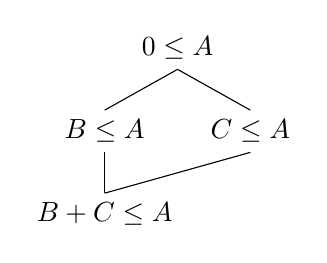
\begin{tikzpicture}[sibling distance=.25cm]
\Tree [.$0\le A$
        [.$B\le A$
            [.\node(BC){$B+C\le A$}; ]]
        [.\node (CA){$C\le A$}; ]] 
\draw (CA.south) -- (BC.north);
\end{tikzpicture}
\\
We can see that multiple nodes can take us to the same children. To break this symmetry we define an ordering that will ensure that a node can have only one parent.
\begin{itemize}
    \item A random ordering is defined for the tensors, for instance we can define $A \prec B \prec C$.
    \item Similarly we define the ordering of dimensions for each tensor, with the first dimension preceding the second and so on. In our example it would be $m \prec n$ for each tensor.
    \item The final ordering is defined on the operations performed to reach the child node: $\text{Summation over terms} \prec \text{Product over terms} \prec \text{Summation over dimensions}$
\end{itemize}
By using these orderings when generating a child for a node we can remove the redundancy. 
For each node we have a list (L) of highest order tensor, dimension and operation used on the root node to reach that node. For our example above, $L(B+C \le A)=\{C,\text{summation over terms}\}$
To generate a child for this node, one can only use a tensor, dimension or operation which has higher or equal order than the highest order tensor, dimension and operation in L.
This rule eliminates redundancy from the graph. For example in the figure above, now $C\le A$ cannot generate $B+C\le A$ because once we add $C$ to the inequality we can't add $B$ as $B \prec C$

\subsubsection{More Complex Setting}
%\textbf{More Complex Setting:} 
Let us now see what happens if we remove the first assumption which was "mod of the numbers in a tensor is all greater than or equal to one". In this case we divide our tensor set into three categories: (1) Where mod of each number is greater than or equal to 1, denoted by $P_1$, (2) Where mod of each number is less than or equal to 1, denoted by $P_2$, (3) Where mod of some numbers are less than 1 and some are greater than 1, denoted by $P_3$.
\\
Taking a product with any tensor in $P_1$ will give us a child node, while multiplying with a tensor in $P_2$ will give us a parent node and a product with a tensor in $P_3$ will give us a sibling.
% We split the product operations into three different operations: We call it $Prod_1$ if the tensor used is from $P_1$, $Prod_1$ if the tensor used is from $P_2$ and $Prod_3$ for tensors from $P_3$.  
So whenever we add a new term to a node, it must start with the product of all tensors in $P_2$ and then removing tensors one by one in the precedence order defined over tensors will give us the child nodes. So, we split the operation used above to reach the child node by splitting the product into two different ones for this setting:
\begin{itemize}
\item $\exists \ \overline{\TX}',\overline{\TX} \in E',E \quad s.t. \  \overline{\TX}' \supseteq \overline{\TX}$ and $\overline{\TX}' \setminus \overline{\TX} \in P_1 $, increase the product by multiplying with a good tensor.
\item $\exists \ \overline{\TX}',\overline{\TX} \in E',E \quad s.t. \ \overline{\TX}' \subseteq \overline{\TX}$ and $\overline{\TX} \setminus \overline{\TX}' \in P_2$, increase the product by removing a bad tensor.
\end{itemize}
The new precedence relationship among the operators is:
$\text{Summation over terms} \prec \text{Removing a bad tensor} \prec \text{Multiplying a good tensor} \prec \text{Summation over dimensions}$


\subsection{Generalization}
Before discussing the removal of the second assumption let us consider a generalization of the structure defined in Eq~\ref{eq:struct}. The main idea behind this generalization is to be able to use negative tensors and subtractions. If we take Eq~\ref{eq:struct} and allow the possibility of taking negation of a tensor we get the following generalization:
%\begin{equation}
%	\displaystyle\sum\limits_{\overline{\TX}_i \in \TE}\bigotimes_{\textbf{S}_i}(\overline{\TX}_i,\overline{\TM}_i) \le \TZ_{M}
%\end{equation}
%
%\begin{equation}
%	\displaystyle-\sum\limits_{\overline{\TX}_i \in \TE}\bigotimes_{\textbf{S}_i}(\overline{\TX}_i,\overline{\TM}_i) \le \TZ_{M}
%\end{equation}
%
%\begin{equation}
%	\displaystyle\sum\limits_{\overline{\TX}_i \in \TE}\bigotimes_{\textbf{S}_i}(\overline{\TX}_i,\overline{\TM}_i) \geq \TZ_{M}
%\end{equation}
%
%\begin{equation}
%	\displaystyle-\sum\limits_{\overline{\TX}_i \in \TE}\bigotimes_{\textbf{S}_i}(\overline{\TX}_i,\overline{\TM}_i) \geq \TZ_{M}
%\end{equation}

\begin{equation}
\label{eq:general1}
	\displaystyle\sum\limits_{\overline{\TX}_i \in \TE}\bigotimes_{\textbf{S}_i}(\overline{\TX}_i,\overline{\TM}_i) - 
	\sum\limits_{\overline{\TX}'_i \in \TE'}\bigotimes_{\textbf{S}'_i}(\overline{\TX}'_i,\overline{\TM}'_i) \le \TZ_{M}
\end{equation}

\begin{equation}
\label{eq:general2}
	\displaystyle\TZ_{M} \le \sum\limits_{\overline{\TX}_i \in \TE}\bigotimes_{\textbf{S}_i}(\overline{\TX}_i,\overline{\TM}_i) - 
	\sum\limits_{\overline{\TX}'_i \in \TE'}\bigotimes_{\textbf{S}'_i}(\overline{\TX}'_i,\overline{\TM}'_i) 
\end{equation}

%\begin{multline}
%\label{eq:genStruct}
%	\displaystyle\TZ_{M} \le \sum\limits_{\overline{\TX}_i \in \TE}\bigotimes_{\textbf{S}_i}(\overline{\TX}_i,\overline{\TM}_i) - 
%	\sum\limits_{\overline{\TX}'_i \in \TE'}\bigotimes_{\textbf{S}'_i}(\overline{\TX}'_i,\overline{\TM}'_i) \le \TZ'_{M'}\\ \forall \bigcup_{E \bigcup E'}(\bigcup_{\TM \in \overline{\TM}_i} \TM / \textbf{S}_i) \bigcup M  \bigcup M' 
%\end{multline}
For now let us focus on learning constraints defined by the structure in Eq~\ref{eq:general1}, we will update our algorithm later to include Eq~\ref{eq:general2}.   
If a tensor \TX is in any element of \TE it's being considered as is while if it belongs to any element of \TE' it's negation is being considered. \TX can also belong to both \TE and \TE', in which case it's being considered in both the states positive and it's negation. 
Now let's say we have a tensor in our data set with all numbers non-positive, then we can take a negation and make it non-negative and use this transformed tensor in our algorithm without any loss of information because the enumeration is going to consider both the tensor and it's negation as explained above.
So we can relax one more assumption we had, we assumed that each tensor must have all numbers non-negative, but now we can also have tensors that have all numbers non-positive. To do the intelligent enumeration, we will have to re-define the concept of most general node and the rules to go to a child node.
The most general node will have the following property now:
\begin{itemize}
\item $E=\phi$
\item $|E'|=2$
\item $|\overline{\TX}'|=2 \quad \forall \, \overline{\TX}' \in E'$ 
\item $\displaystyle S'_i = \bigcup_{\TM \in \overline{M}'_i} M \quad \forall \, \overline{M}'_i \in E'$
\end{itemize}



\subsection{Bringing it all together}
We will use the bottom up approach, so we start with the most specific constraint and if it's satisfied we consider all it's children and if not we remove it and all it's descendants, we will define a total ordering on the set of constraints to remove redundancy when enumerating as multiple nodes can have same children. To define ordering we are going to separate Eq~\ref{eq:struct}: the positive one and the negative one.
\\
A positive term can be made more general by doing one of the following:
\begin{itemize}
\item $|E'| > |E|$, adding more positive terms
\item $\exists l'\in E \quad s.t. \quad  |l'| < |l|$, adding more products 
\item $\exists S'_l\in E \quad s.t. \quad S'_l \subset S_l$, summing over more dimensions
\end{itemize}
A negative term can be made more general by doing one of the following:
\begin{itemize}
\item $|F'| < |F|$, removing negative terms
\item $\exists l'\in F \quad s.t. \quad  |l'| > |l|$, removing products 
\item $\exists S'_l\in F \quad s.t. \quad S'_l \supseteq S_l$, summing over less dimensions
\end{itemize}
We define a node $n'$  to be a child of another node $n$ if and only if either $n'$ has a positive node that is child of another positive node in $n$ or $n'$ has a negative node that is child of another negative node in $n$ but never both.


\bibliographystyle{unsrt}
\bibliography{ijcai18}
\end{document}